% hack to deal with beamer/pgf bug
\RequirePackage{atbegshi}

\documentclass{beamer}% This is the file main.tex


% blackboard symbols

\newcommand{\C}{\ensuremath{\mathbb{C}}}
\newcommand{\D}{\ensuremath{\mathbb{D}}}
\newcommand{\F}{\ensuremath{\mathbb{F}}}
\newcommand{\G}{\ensuremath{\mathbb{G}}}
\newcommand{\J}{\ensuremath{\mathbb{J}}}
\newcommand{\N}{\ensuremath{\mathbb{N}}}
\newcommand{\Q}{\ensuremath{\mathbb{Q}}}
\newcommand{\R}{\ensuremath{\mathbb{R}}}
\newcommand{\T}{\ensuremath{\mathbb{T}}}
\newcommand{\Z}{\ensuremath{\mathbb{Z}}}

\newcommand{\Zt}{\ensuremath{\Z_t}}
\newcommand{\Zp}{\ensuremath{\Z_p}}
\newcommand{\Zq}{\ensuremath{\Z_q}}
\newcommand{\ZN}{\ensuremath{\Z_N}}
\newcommand{\Zps}{\ensuremath{\Z_p^*}}
\newcommand{\ZNs}{\ensuremath{\Z_N^*}}
\newcommand{\JN}{\ensuremath{\J_N}}
\newcommand{\QRN}{\ensuremath{\mathbb{QR}_N}}

% "left-right" pairs of symbols

% inner product
\newcommand{\inner}[1]{\langle{#1}\rangle}
\newcommand{\innerfit}[1]{\left\langle{#1}\right\rangle}
% absolute value
\newcommand{\abs}[1]{\lvert{#1}\rvert}
\newcommand{\absfit}[1]{\left\lvert{#1}\right\rvert}
% a set
\newcommand{\set}[1]{\{{#1}\}}
\newcommand{\setfit}[1]{\left\{{#1}\right\}}
% parens
\newcommand{\parens}[1]{({#1})}
\newcommand{\parensfit}[1]{\left({#1}\right)}
% tuple, alias for parens
\newcommand{\tuple}[1]{\parens{#1}}
\newcommand{\tuplefit}[1]{\parensfit{#1}}
% square brackets
\newcommand{\bracks}[1]{[{#1}]}
\newcommand{\bracksfit}[1]{\left[{#1}\right]}
% rounding off
\newcommand{\round}[1]{\lfloor{#1}\rceil}
\newcommand{\roundfit}[1]{\left\lfloor{#1}\right\rceil}
% floor function
\newcommand{\floor}[1]{\lfloor{#1}\rfloor}
\newcommand{\floorfit}[1]{\left\lfloor{#1}\right\rfloor}
% ceiling function
\newcommand{\ceil}[1]{\lceil{#1}\rceil}
\newcommand{\ceilfit}[1]{\left\lceil{#1}\right\rceil}
% length of some vector, element
\newcommand{\length}[1]{\lVert{#1}\rVert}
\newcommand{\lengthfit}[1]{\left\lVert{#1}\right\rVert}


% macros for matrices and vectors
\newcommand{\matA}{\ensuremath{\mathbf{A}}}
\newcommand{\matB}{\ensuremath{\mathbf{B}}}
\newcommand{\matC}{\ensuremath{\mathbf{C}}}
\newcommand{\matD}{\ensuremath{\mathbf{D}}}
\newcommand{\matE}{\ensuremath{\mathbf{E}}}
\newcommand{\matF}{\ensuremath{\mathbf{F}}}
\newcommand{\matG}{\ensuremath{\mathbf{G}}}
\newcommand{\matH}{\ensuremath{\mathbf{H}}}
\newcommand{\matI}{\ensuremath{\mathbf{I}}}
\newcommand{\matJ}{\ensuremath{\mathbf{J}}}
\newcommand{\matK}{\ensuremath{\mathbf{K}}}
\newcommand{\matL}{\ensuremath{\mathbf{L}}}
\newcommand{\matM}{\ensuremath{\mathbf{M}}}
\newcommand{\matN}{\ensuremath{\mathbf{N}}}
\newcommand{\matO}{\ensuremath{\mathbf{O}}}
\newcommand{\matP}{\ensuremath{\mathbf{P}}}
\newcommand{\matQ}{\ensuremath{\mathbf{Q}}}
\newcommand{\matR}{\ensuremath{\mathbf{R}}}
\newcommand{\matS}{\ensuremath{\mathbf{S}}}
\newcommand{\matT}{\ensuremath{\mathbf{T}}}
\newcommand{\matU}{\ensuremath{\mathbf{U}}}
\newcommand{\matV}{\ensuremath{\mathbf{V}}}
\newcommand{\matW}{\ensuremath{\mathbf{W}}}
\newcommand{\matX}{\ensuremath{\mathbf{X}}}
\newcommand{\matY}{\ensuremath{\mathbf{Y}}}
\newcommand{\matZ}{\ensuremath{\mathbf{Z}}}
\newcommand{\matzero}{\ensuremath{\mathbf{0}}}

\newcommand{\veca}{\ensuremath{\mathbf{a}}}
\newcommand{\vecalpha}{\ensuremath{\mathbf{\alpha}}}
\newcommand{\vecb}{\ensuremath{\mathbf{b}}}
\newcommand{\vecc}{\ensuremath{\mathbf{c}}}
\newcommand{\vecd}{\ensuremath{\mathbf{d}}}
\newcommand{\vece}{\ensuremath{\mathbf{e}}}
\newcommand{\vecf}{\ensuremath{\mathbf{f}}}
\newcommand{\vecg}{\ensuremath{\mathbf{g}}}
\newcommand{\vech}{\ensuremath{\mathbf{h}}}
\newcommand{\veck}{\ensuremath{\mathbf{k}}}
\newcommand{\vecm}{\ensuremath{\mathbf{m}}}
\newcommand{\vecp}{\ensuremath{\mathbf{p}}}
\newcommand{\vecq}{\ensuremath{\mathbf{q}}}
\newcommand{\vecr}{\ensuremath{\mathbf{r}}}
\newcommand{\vecs}{\ensuremath{\mathbf{s}}}
\newcommand{\vect}{\ensuremath{\mathbf{t}}}
\newcommand{\vecu}{\ensuremath{\mathbf{u}}}
\newcommand{\vecv}{\ensuremath{\mathbf{v}}}
\newcommand{\vecw}{\ensuremath{\mathbf{w}}}
\newcommand{\vecx}{\ensuremath{\mathbf{x}}}
\newcommand{\vecy}{\ensuremath{\mathbf{y}}}
\newcommand{\vecz}{\ensuremath{\mathbf{z}}}
\newcommand{\veczero}{\ensuremath{\mathbf{0}}}

\DeclareMathOperator{\diag}{diag}
\renewcommand{\O}{\mathcal{O}}

%% BOILERPLATE PRESENTATION STUFF

% an underlining package
\usepackage{ulem}
% use normal italics for emphasis
\normalem

% my custom theme
\usetheme{CJP}

% dingbats
\usepackage{pifont}

\renewcommand{\Check}{\ding{52}}
\newcommand{\Cross}{\ding{55}}
\newcommand{\Hand}{\ding{43}}
\newcommand{\GreenCheck}{{\color{Green}\Check}}
\newcommand{\RedCross}{{\color{Red}\Cross}}
\newcommand{\Orange}[1]{{\color{Orange} #1}}

% alias for citations
\newcommand{\citationsize}{\footnotesize}

\subject{Theoretical Computer Science}

% suppress ugly QEDs in proofs
\def\qedsymbol{}


% regular lwe was screwing up for some reason
\newcommand{\mylwe}{\textsf{LWE}}

% cal shorthands
\newcommand{\calI}{\mathcal{I}}
\newcommand{\calF}{\mathcal{F}}

% To emphasize short, uniform 
\newcommand{\short}[1]{\ensuremath{{\color{red} #1}}}
\newcommand{\unif}[1]{\ensuremath{{\color{blue} #1}}}

% Citing references smaller but to change in one place if too small
\newcommand{\inlinecite}[1]{{\footnotesize [#1]}}


% GENERAL COMPUTING STUFF (from Chris minus what doesn't work)

\newcommand{\bit}{\ensuremath{\set{0,1}}}
\newcommand{\pmone}{\ensuremath{\set{-1,1}}}

% asymptotic stuff
\DeclareMathOperator{\poly}{poly}
\DeclareMathOperator{\polylog}{polylog}
\DeclareMathOperator{\negl}{negl}
\newcommand{\Otil}{\ensuremath{\tilde{O}}}

% probability/distribution stuff
\DeclareMathOperator*{\E}{\mathbb{E}}
\DeclareMathOperator*{\Var}{Var}

% assorted
\DeclareMathOperator*{\wt}{wt}

% hash functions
\newcommand{\calH}{\ensuremath{\mathcal{H}}}
\newcommand{\calX}{\ensuremath{\mathcal{X}}}
\newcommand{\calY}{\ensuremath{\mathcal{Y}}}

\newcommand{\compind}{\ensuremath{\stackrel{c}{\approx}}}
\newcommand{\statind}{\ensuremath{\stackrel{s}{\approx}}}
\newcommand{\perfind}{\ensuremath{\equiv}}

% font for general-purpose algorithms
\newcommand{\algo}[1]{\ensuremath{\mathsf{#1}}\xspace}

% font for general-purpose computational problems
%\iflncs
%\renewcommand{\problem}[1]{\ensuremath{\mathsf{#1}}\xspace}
%\else
%\newcommand{\problem}[1]{\ensuremath{\mathsf{#1}}\xspace}
%\fi

% font for complexity classes
\newcommand{\class}[1]{\ensuremath{\mathsf{#1}}\xspace}

% complexity classes and languages
\renewcommand{\P}{\class{P}}
\newcommand{\BPP}{\class{BPP}}
\newcommand{\NP}{\class{NP}}
\newcommand{\coNP}{\class{coNP}}
\newcommand{\AM}{\class{AM}}
\newcommand{\coAM}{\class{coAM}}
\newcommand{\IP}{\class{IP}}
\newcommand{\SZK}{\class{SZK}}
\newcommand{\NISZK}{\class{NISZK}}
\newcommand{\NICZK}{\class{NICZK}}
\newcommand{\PPP}{\class{PPP}}
\newcommand{\PPAD}{\class{PPAD}}

\newcommand{\yes}{\ensuremath{\text{YES}}}
\newcommand{\no}{\ensuremath{\text{NO}}}

\newcommand{\Piyes}{\ensuremath{\Pi^{\yes}}}
\newcommand{\Pino}{\ensuremath{\Pi^{\no}}}
 % commands for these slides only 
% additional libraries for tikz and pgf
\usepackage{tikz}
\usetikzlibrary{matrix}
\usetikzlibrary{calc}
\usetikzlibrary{shadows}
\usetikzlibrary{scopes}
\usetikzlibrary{chains}
\usetikzlibrary{positioning}
\usetikzlibrary{fit}
\usetikzlibrary{backgrounds}
\usetikzlibrary{decorations.pathmorphing}
\usetikzlibrary{decorations.pathreplacing}
\usetikzlibrary{shapes.geometric}
\usetikzlibrary{shapes.symbols}
\usetikzlibrary{shapes.misc}
\usetikzlibrary{trees}

% color aliases
%\colorlet{Lattice}{Green}
%\colorlet{Set}{Red!10}

% global styles
\tikzset{
  % make drop shadows a bit softer
  every shadow/.style={opacity=.4,shadow xshift=.3ex,shadow yshift=-.3ex},
  % use \& to separate cells in matrices, avoiding fragility in beamer frames
  every matrix/.style={ampersand replacement=\&},
  % edges and joins with arrows and thicker
  every edge/.append style={->,thick},
  every join/.style={->,thick},
  % distance between nodes
  % node distance=1ex and 2ex,
}

% styles for drawing in Rn, especially lattices
\tikzset{
  % lattice transform must include "cm" dimension to work properly,
  % otherwise the x and y transforms become dependent
  Ztrans/.style={x={(1.5cm,1cm)},y={(.5cm,1.5cm)}},
  Zdual/.style={x={(1.5cm,-.5cm)},y={(.5cm,1cm)}},
  latttrans/.style={x={(1.8cm,.5cm)},y={(0.4cm,1.3cm)}},
  dualtrans/.style={x={(1.3cm,-.4cm)},y={(-.5cm,1.8cm)}},
  lattB/.style={x={(1.8cm,.5cm)},y={(0.4cm,1.4cm)}},
  dualB/.style={x={(1.4cm,-.4cm)},y={(-.5cm,1.8cm)}},
  shortB/.style={x={(.5cm,.2cm)},y={(-.1cm,1.7cm)}},
  latt2B/.style={x={(1cm,.1cm)},y={(.1cm,1.2cm)}},
  ulattB/.style={x={(2.0cm,.5cm)},y={(2.1cm,-.2cm)}},
  openball/.style={fill=structure.fg!20},
  ball/.style={openball,thin,draw=structure.fg},
  latt/.style={Lattice,fill},
  dist/.style={Brown,densely dashed,font=\footnotesize},
  offlabel/.style={Brown,inner sep=2pt,font=\tiny},
  axes/.style={->,Gray,style=very thin},
  fundamental/.style={Gray,fill opacity=.2},
  target/.style={fill,Brown},
  project/.style={thin,dashed},
  help lines/.style={Gray,very thin,step=.5cm},
  % expanding waves representing noise
  noise/.style={
    Lattice,
    opacity=.5,
    decorate,decoration={
      expanding waves,
      segment length=5pt,angle=10,
      post=moveto,post length=3pt
    },
  },
}

% lattice that can be dropped into any path.
% it would be sensible to set a default argument here, but
% commands with optional args don't parse correctly inside a
% tikz path
\newcommand*{\latt}[1]{%
  \foreach \a in {-4, ..., 4} {
    \foreach \b in {-4, ..., 4} {
      (\a,\b) circle (#1)
    }
  }
}

% style for functions mapping one point to another
\tikzset{map/.style={->,semithick}}

% style for an offset rounded box
\tikzset{showoff/.style={draw,fill=White,rounded corners,drop
    shadow,inner sep=6pt}}

% style for all algorithms
\tikzset{algorithm/.style={
    draw=#1!50!Black!60,solid,
    top color=White,bottom color=#1!50!Black!15,
    very thick,rounded corners,drop shadow,
    minimum size=.9cm,inner sep=6pt,outer sep=4pt
  }
}

% style for honest, malicious, trusted parties
\tikzset{honest/.style={algorithm=Green}}
\tikzset{oracle/.style={algorithm=Green}}
\tikzset{malicious/.style={algorithm=Red}}
\tikzset{trusted/.style={algorithm=Purple,inner sep=10pt}}

% style for notions
\tikzset{notion/.style={
    draw=#1!50!Black!60,solid,
    top color=White,bottom color=#1!50!Black!15,
    very thick,rounded corners,drop shadow,
    minimum height=6.5ex,inner sep=6pt,
  }
}

\tikzset{app/.style={notion=Blue}}
\tikzset{prim/.style={notion=Green}}
\tikzset{math/.style={notion=Red}}

% % style for a common reference string
\tikzset{crs/.style={draw,fill=White,cloud,cloud puffs=13,cloud ignores aspect,drop shadow}}


% basic notation

\newcommand{\lamperp}{\Lambda^{\perp}}
\newcommand{\lam}{\Lambda}

% lattice
\newcommand{\lat}{\mathcal{L}}
% fundamental region
\newcommand{\piped}{\mathcal{P}}
% smoothing parameter
\newcommand{\smooth}{\eta}
% smoothing w/ epsilon
\newcommand{\smootheps}{\smooth_{\epsilon}}
% ball
\newcommand{\ball}{\mathcal{B}}
% cube
\newcommand{\cube}{\mathcal{C}}
% covering radius symbol
\newcommand{\cover}{\ensuremath{\mu}}
% Gram-Schmidt
\newcommand{\gs}[1]{\ensuremath{\widetilde{#1}}}
% GS minimum
\newcommand{\gsmin}{\ensuremath{\tilde{bl}}}
% volume operation
\DeclareMathOperator{\vol}{vol}
% Hermite normal form
\DeclareMathOperator{\hnf}{HNF}
% rank
\DeclareMathOperator{\rank}{rank}
% distance operator
\DeclareMathOperator{\dist}{dist}
% span operator
\DeclareMathOperator{\spn}{span}
% error function
\DeclareMathOperator{\erf}{erf}

% quantities that show up regularly
\newcommand{\wsln}{\ensuremath{\omega(\sqrt{\log n})}}
\newcommand{\wslm}{\ensuremath{\omega(\sqrt{\log m})}}

% support algorithms
\newcommand{\sampleZ}{\algo{Sample}\Z}
\newcommand{\sampleD}{\algo{SampleD}}
\newcommand{\tobasis}{\algo{ToBasis}}
\newcommand{\invert}{\algo{Invert}}
\newcommand{\genbasis}{\algo{GenBasis}}
\newcommand{\extbasis}{\algo{ExtBasis}}
\newcommand{\extlattice}{\algo{ExtLattice}}
\newcommand{\randbasis}{\algo{RandBasis}}
\newcommand{\gentrap}{\algo{GenTrap}}
\newcommand{\deltrap}{\algo{DelTrap}}
\newcommand{\noisy}{\algo{Noisy}}

% problems related to lattices
\newcommand{\svp}{\problem{SVP}}
\newcommand{\gapsvp}{\problem{GapSVP}}
\newcommand{\cogapsvp}{\problem{coGapSVP}}
\newcommand{\usvp}{\problem{uSVP}}
\newcommand{\sivp}{\problem{SIVP}}
\newcommand{\gapsivp}{\problem{GapSIVP}}
\newcommand{\cvp}{\problem{CVP}}
\newcommand{\gapcvp}{\problem{GapCVP}}
\newcommand{\cvpp}{\problem{CVPP}}
\newcommand{\gapcvpp}{\problem{GapCVPP}}
\newcommand{\bdd}{\problem{BDD}}
\newcommand{\gdd}{\problem{GDD}}
\newcommand{\add}{\problem{ADD}}
\newcommand{\incgdd}{\problem{IncGDD}}
\newcommand{\incivd}{\problem{IncIVD}}
\newcommand{\crp}{\problem{CRP}}
\newcommand{\gapcrp}{\problem{GapCRP}}
% problems on ideal lattices
\newcommand{\igvp}{\problem{IGVP}}
\newcommand{\incigvp}{\problem{IncIGVP}}
% avg-case stuff
\newcommand{\sis}{\problem{SIS}}
\newcommand{\isis}{\problem{ISIS}}
\newcommand{\ilwe}{\problem{ILWE}}
\newcommand{\lwe}{\problem{LWE}}
\newcommand{\rlwe}{\problem{RLWE}}
\newcommand{\lwr}{\problem{LWR}}
\newcommand{\rlwr}{\problem{RLWR}}
\newcommand{\dlwe}{\problem{DLWE}}
\newcommand{\lpn}{\problem{LPN}}
\newcommand{\Psibar}{\ensuremath{\bar{\Psi}}}

% crypto-related notation

% KEYS AND RELATED

\newcommand{\mm}[1]{\ensuremath{#1}}

\newcommand{\pp}{\mm{pp}}      % public params
\newcommand{\pk}{\mm{pk}}
\newcommand{\vk}{\mm{vk}}
\newcommand{\sk}{\mm{sk}}
\newcommand{\mpk}{\mm{mpk}}
\newcommand{\msk}{\mm{msk}}
\newcommand{\fk}{\mm{fk}}
\newcommand{\id}{id}
\newcommand{\msgspace}{\ensuremath{\mathcal{M}}}
\newcommand{\idspace}{\ensuremath{\mathcal{ID}}}

\newcommand{\concat}{\ensuremath{\|}}

% GAMES STUFF

% advantage
\newcommand{\advan}{\ensuremath{\mathbf{Adv}}}

% different attack models
\newcommand{\attack}[1]{\ensuremath{\text{#1}}}

\newcommand{\atk}{\attack{atk}} % dummy attack
\newcommand{\indcpa}{\attack{ind-cpa}}
\newcommand{\indcca}{\attack{ind-cca}}
\newcommand{\anocpa}{\attack{ano-cpa}} % anonymous
\newcommand{\anocca}{\attack{ano-cca}}
\newcommand{\sidindcpa}{\attack{sid-ind-cpa}} % selective-id
\newcommand{\aidindcpa}{\attack{aid-ind-cpa}} % adaptive-id
\newcommand{\sidindcca}{\attack{sid-ind-cca}}
\newcommand{\aidindcca}{\attack{aid-ind-cca}}
\newcommand{\euacma}{\attack{eu-acma}} % forgery: adaptive chosen-message
\newcommand{\euscma}{\attack{eu-scma}} % forgery: static chosen-message
\newcommand{\suacma}{\attack{su-acma}} % strong forgery: adaptive chosen-message
\newcommand{\suscma}{\attack{su-scma}} % strong forgery: static chosen-message

% ADVERSARIES
\newcommand{\attacker}[1]{\ensuremath{\mathcal{#1}}}

\newcommand{\Adv}{\attacker{A}}
\newcommand{\Sim}{\attacker{S}}
\newcommand{\Ora}{\attacker{O}}
\newcommand{\Inv}{\attacker{I}}
\newcommand{\For}{\attacker{F}}

% CRYPTO SCHEMES

\newcommand{\scheme}[1]{\ensuremath{\text{#1}}}

% public-key cryptosystem
\newcommand{\pkc}{\scheme{PKC}}
\newcommand{\pkcsetup}{\algo{Setup}}
\newcommand{\pkcgen}{\algo{Gen}}
\newcommand{\pkcenc}{\algo{Enc}} % can also use \kemenc and \kemdec
\newcommand{\pkcdec}{\algo{Dec}}
\newcommand{\msgsp}{\mathcal{M}}

% extra deniable algorithms for pkc
\newcommand{\biden}{\scheme{BI\mbox{-}DEN}}
\newcommand{\den}{\scheme{DEN}}
\newcommand{\dengen}{\algo{DenGen}} 
\newcommand{\denenc}{\algo{DenEnc}} % can also use \kemenc and \kemdec
\newcommand{\rfake}{\algo{RecFake}}
\newcommand{\sfake}{\algo{SendFake}}

% plan ahead deniability 
\newcommand{\pden}{\scheme{PL\mbox{-}DEN}}
\newcommand{\pdenenc}{\algo{PADenEnc}} % can also use \kemenc and \kemdec
\newcommand{\prfake}{\algo{PARecFake}}
\newcommand{\psfake}{\algo{PASendFake}}

% bitranslucent sets
\newcommand{\bts}{\scheme{BTS}}
\newcommand{\btsgen}{\algo{Gen}}
\newcommand{\btsdengen}{\algo{DenGen}}
\newcommand{\sampleP}{\algo{SampleP}} 
\newcommand{\sampleU}{\algo{SampleU}} 
\newcommand{\testP}{\algo{TestP}}
\newcommand{\fakeScoins}{\algo{FakeSCoins}}
\newcommand{\fakeRcoins}{\algo{FakeRCoins}}

% digital signatures
\newcommand{\sig}{\scheme{SIG}}
\newcommand{\siggen}{\algo{Gen}}
\newcommand{\sigsign}{\algo{Sign}}
\newcommand{\sigver}{\algo{Ver}}

% key-encapsulation mechanism
\newcommand{\kem}{\scheme{KEM}}
\newcommand{\kemgen}{\algo{Gen}}
\newcommand{\kemenc}{\algo{Encaps}}
\newcommand{\kemdec}{\algo{Decaps}}

% symmetric cipher
\newcommand{\sym}{\scheme{SYM}}
\newcommand{\symenc}{\algo{E}}
\newcommand{\symdec}{\algo{D}}

% identity-based encryption
\newcommand{\ibe}{\scheme{IBE}}
\newcommand{\ibesetup}{\algo{Setup}}
\newcommand{\ibeext}{\algo{Ext}}
\newcommand{\ibeenc}{\algo{Enc}}
\newcommand{\ibedec}{\algo{Dec}}

% hierarchical IBE (as key encapsulation)
\newcommand{\hibe}{\scheme{HIBE}}
\newcommand{\hibesetup}{\algo{Setup}}
\newcommand{\hibeext}{\algo{Extract}}
\newcommand{\hibeenc}{\algo{Encaps}}
\newcommand{\hibedec}{\algo{Decaps}}

% binary tree encryption (as key encapsulation)
\newcommand{\bte}{\scheme{BTE}}
\newcommand{\btesetup}{\algo{Setup}}
\newcommand{\bteext}{\algo{Extract}}
\newcommand{\bteenc}{\algo{Encaps}}
\newcommand{\btedec}{\algo{Decaps}}

% trapdoor functions
\newcommand{\tdf}{\scheme{TDF}}
\newcommand{\tdfgen}{\algo{Gen}}
\newcommand{\tdfeval}{\algo{Eval}}
\newcommand{\tdfinv}{\algo{Invert}}
\newcommand{\tdfver}{\algo{Ver}}

% preimage samplable functions
\newcommand{\psf}{\scheme{PSF}}
\newcommand{\psfgen}{\algo{Gen}}
\newcommand{\psfsamdom}{\algo{SampleDom}}
\newcommand{\psfsampre}{\algo{SamplePre}}

% COMPLEXITY MEASURES

\newcommand{\qhash}{\ensuremath{Q_{H}}}
\newcommand{\qext}{\ensuremath{Q_{E}}}
\newcommand{\qid}{\ensuremath{Q_{\text{id}}}}
\newcommand{\qsign}{\ensuremath{Q_{\text{sign}}}}

% UC STUFF

\newcommand{\func}[1]{\ensuremath{\mathcal{F}_{#1}}\xspace}
\newcommand{\prot}[1]{\ensuremath{\mathcal{\pi}_{#1}}\xspace}
\newcommand{\exec}{\ensuremath{\text{EXEC}}}
\newcommand{\ideal}{\ensuremath{\text{IDEAL}}}
% \Sim and \Adv are already defined above
\newcommand{\Env}{\attacker{Z}}
\newcommand{\sid}{\ensuremath{\mathsf{sid}}\xspace}
\newcommand{\ssid}{\ensuremath{\mathsf{ssid}}\xspace}
\newcommand{\command}[1]{\ensuremath{\mathsf{#1}}\xspace}
\title{Circular and KDM Security for Identity-Based Encryption}

\newif\ifnotes\notesfalse

\ifnotes
\newcommand{\jnote}[1]{{\bf (\color{red}{Jacob:}} {#1}{\bf ) }}
\newcommand{\cnote}[1]{{\bf (\color{blue}{Chris:}} {#1}{\bf ) }}
\else
\newcommand{\jnote}[1]{}
\newcommand{\cnote}[1]{}
\fi

\author{%
  Jacob Alperin-Sheriff\footnotemark[1]  %
  %
}
\institute{\footnotemark[1]based on work with Chris Peikert}
\date{\today}
\begin{document}
\begin{frame}[label=title]
\titlepage
\end{frame}
\section*{Outline}
\begin{frame}{Notions of Security for Encryption Schemes}
\begin{figure}
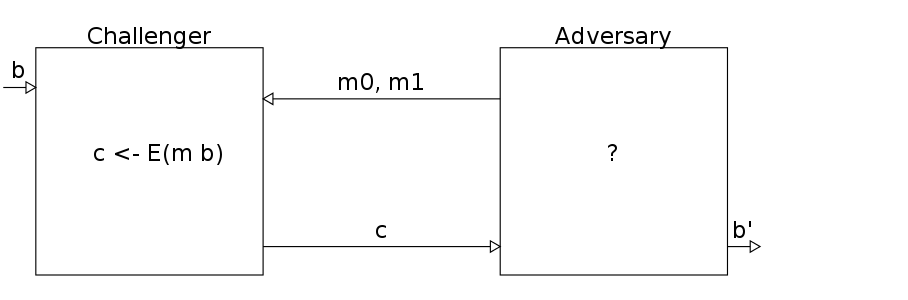
\includegraphics[width=.85\textwidth]{ss.png}
\end{figure}
\begin{itemize}
\item<+-> Basic notion of security--\alert{semantic security} \inlinecite{GM'82}.
\begin{itemize}
\item<.-> Security game paramterized by bit $b$ (unknown to adversary)
\item<.-> Adversary is given public parameters (if any)
\item<.-> Can send challenger two messages $m_0$ and $m_1$ of \onslide*<1-2>{her choice}\onslide*<3->{\alert{\textbf{her choice}}}
\item<.-> Receives encryption of message $m_b$
\end{itemize}
\item<+-> For security, adversary must be able guess $b$ with probability at most negligibly greater than $1/2$.
\item<+-> Adversary cannot receive encryptions of key-dependent messages. 
\item<+-> Can plaintexts ever be key-dependent? 
\end{itemize}
\end{frame}
\begin{frame}{Circular and Key-Dependent Message Security}
  \begin{figure}
    \jnote{FIX: Label either via LaTex or picture Alice, Bob, put Eve
      in there somewhere and make a biblical funny, i.e.  ciphertext
      is the fruit}
    
\includegraphics[width=.25\textwidth]{circularsecuresnake2.png}
  \end{figure}
  \begin{block}{Can Plaintext Be Key-Dependent?}
    \begin{itemize}
    \item<+-> Yes!
      \begin{itemize}
      \item<.-> Careless or Improper key management
      \item<.-> Integral part of cryptosystem: Gentry's
        ``bootstrapping'' for FHE requires circular-security of secret
        key \inlinecite{Gentry'09}
      \end{itemize}
    \item<+-> Previous results in KDM-security focused on \alert{symmetric}
      and \alert{public-key} encryption and applications, e.g
      \inlinecite{BHHO'08 (DDH), HH'09, ACPS'09 (LWE),BG'10 (QR),
        App'11, MTY'11, BGK'11,BV'11}
    \end{itemize}
  \end{block}

\end{frame}

  \begin{frame}{KDM Attack Model}
    \begin{enumerate}
    \item<1-> Challenger parameterized by bit $b$:\\ sends adversary
      public keys of $d$ arbitrary users
    \item<2-> Adversary makes key-dependent message queries
      \begin{itemize}
      \item<3-> Note: Single-message and multiple-message models
        \alert{NOT} equivalent
      \end{itemize}
    \item<4-> Adversary eventually outputs guess $b'$
    \end{enumerate}
    \begin{figure}
      \begin{tikzpicture}
     
     	% Adversary picture/text
        \pgfdeclareimage[interpolate=true,width=3cm,height=3cm]{adversary}{devil1.png}
        \pgftext[at=\pgfpoint{0cm}{-0.25cm},left,base]{\pgfuseimage{adversary}}
        \pgftext[at=\pgfpoint{.65cm}{-0.3cm},left,base]{Adversary}
        \pgfpathrectangle{\pgfpoint{0.0cm}{-0.5cm}}{\pgfpoint{2.9cm}{3.25cm}}

        % \pgftext[at=\pgfpoint{1.2cm}{0.05cm},left,base]{A}
        
        % Challenger picture/text 
                \pgfpathrectangle{\pgfpoint{7cm}{-0.5cm}}{\pgfpoint{3.5cm}{3.25cm}} % Box
        \pgftext[at=\pgfpoint{7.65cm}{-0.3cm},left,base]{Challenger($b$)}
        \pgftext[at=\pgfpoint{7.7cm}{1.5cm},left,base]{$
          pk_1, \ldots, pk_d$}
         \pgftext[at=\pgfpoint{7.7cm}{1.0cm},left,base]{$sk_1, \ldots, sk_d$}




    %    \pgfpathrectangle{\pgfpoint{6.75cm}{1cm}}{\pgfpoint{3cm}{1cm}} % Encryption box
       	% public keys sent to adversary
        \pgfusepath{stroke} 
        
        
        \onslide<1|handout:0>{ \draw[->,line
          width=0.05cm] (7.00cm, 1.2cm) -- (2.9cm, 1.2cm)
          node[midway,above] {$pk_1, \ldots, pk_d$}; }
          
         % Sends first function 
        \onslide<2-3|handout:1>{ \draw[->, line width=0.05cm] (2.9cm,
          2.2cm) -- (7.00cm, 2.2cm) node[midway, above]{$\scriptstyle f_0, f_1,
            \text{user } i$};

       
          \draw[->, line width=0.05cm] (7.00cm,1.55cm) --     (2.9, 1.55cm)
          node[midway, above]{$\scriptstyle
            c_{f}=\text{Enc}_{pk_{i}}(f_{b}( sk_1, \ldots, sk_{d}))$};     
 
        }

        \onslide<3|handout:0>{ \draw[->, line width=0.05cm] (2.9cm,
          0.5cm) -- (7.00cm, 0.5cm) node[midway, above]{$\scriptstyle g_0, g_1,
            \text{user } j$};

          \draw[->, line width=0.05cm] (7.00cm,-0.15cm) -- (2.9cm,
          -0.15cm) node[midway, above]{$\scriptstyle
            c_{g}=\text{Enc}_{pk_{j}}(g_{b}( sk_1, \ldots, sk_{d}))$};


        }

        \onslide<4-|handout:0>{ \draw[->,line width=0.05cm] (2.9cm,
          1cm) -- (5cm, 1cm) node[midway, above]{$b'$}; }

      \end{tikzpicture}
    \end{figure}

  \end{frame}

\begin{frame}{Identity-Based Encryption}
\begin{itemize}
\item<+-> Normal public-key encryption
\begin{itemize}
\item<.-> Public keys unrelated to a
  user's identity
\smallskip
\item<.-> Requires cumbersome public key infrastructure, certificates
\end{itemize}
\item<+-> Identity-based encryption
\begin{itemize}
\item<.-> Public keys are user's identities,
  i.e. \textsf{jmas6@cc.gatech.edu}
\smallskip
\item<.-> Private key generator with master secret key generates user
  secret keys
\end{itemize}
\item<+-> Security for Identity-Based Encryption
\begin{itemize}
\item<.-> Adversary may request secret keys for identities of her
  choice
\smallskip
\item<+-> \alert{Selective Security}-Adversary must specify identity
  to attack before seeing any public parameters of scheme
\smallskip
\item<+-> \alert{Adaptive Security}-Adversary may request secret keys
before specifying the challenge identity
\end{itemize}
\end{itemize}
\end{frame}



\begin{frame}{KDM Security for Identity-Based Encryption}
Key-dependent messages arise naturally in identity-based encryption
  \begin{itemize}
  \item<+-> IBE for revocation: user identity at epoch
    $i$ is $\text{id} := \text{username}||i$\\
 PKG sends key for next epoch by encrypting it under
    previous identity.
  \item<+-> What if user deleted old key, wants to decrypt old
    ciphertext?
  \item<+-> Solution: PKG sends old key encrypted under
    current epoch's identity.
  \item<+-> May be unsafe if the IBE is not KDM-secure
  \end{itemize}
  \begin{overprint}
  \begin{figure}
    \begin{tikzpicture}
      \definecolor{superlightblue}{rgb}{0.7,0.8,1}
      \definecolor{lightblue}{rgb}{0.4,0.6,1}
      \pgfdeclareimage[interpolate=true,width=2cm,height=2cm]{bobhappy}{bobhappy.png}
      \pgfdeclareimage[interpolate=true,width=2cm,height=2cm]{bobsad}{bobsad.png}
      \pgfdeclareimage[interpolate=true,width=2cm,height=2cm]{bobunsure}{bobunsure.png}
      \draw [draw=black, line width=.05cm] (8cm,0cm)
      rectangle (11cm, 3cm); 
      
      \draw [draw=black, line width=.05cm] (-0.2cm,0cm) rectangle (2.3cm, 3cm);
      \onslide*<1,3|handout:0>{\pgftext[at=\pgfpoint{0cm}{0.4cm},left,base]{\pgfuseimage{bobhappy}}
      }
      \onslide*<2|handout:0>{\pgftext[at=\pgfpoint{0cm}{0.4cm},left,base]{\pgfuseimage{bobunsure}}
      }
      \onslide*<4|handout:1>{\pgftext[at=\pgfpoint{0cm}{0.4cm},left,base]{\pgfuseimage{bobsad}}
      }


      \pgftext[at=\pgfpoint{8.25cm}{1.6cm},left,base]{\Large Private
        Key} \pgftext[at=\pgfpoint{8.4cm}{1.1cm},left,base]{\Large
        Generator}

      \draw[<-, line width=.1cm,black] (2.4cm, 1.5cm) -- (7.9cm,
      1.5cm);

      \onslide<1|handout:0>{\pgftext[at=\pgfpoint{0.15cm}{2.6cm},left,base]{\large
          Bob$||$March}

        \pgftext[at=\pgfpoint{-0.1cm}{0.1cm},left,base]{\scriptsize
          $sk$ for Bob$||$March} }


      \onslide<2-4|handout:1>{\pgftext[at=\pgfpoint{0.15cm}{2.6cm},left,base]{\large
          Bob$||$April}

        \pgftext[at=\pgfpoint{-0.1cm}{0.1cm},left,base]{\scriptsize
          $sk$ for Bob$||$April} } 
          
          \onslide<1-4>{ \filldraw
        [draw=lightblue, line width=.35cm, rounded corners,
        fill=superlightblue] (3.5cm,0.2cm) rectangle (7cm,1.2cm);

	\pgftext[at=\pgfpoint{5.45cm}{0.12cm},left,base]{\scriptsize
          Bob$||$March}
	
	\pgftext[at=\pgfpoint{3.55cm}{1.12cm},left,base]{\scriptsize
          Bob$||$March} } 


      \onslide<1-4|handout:1>{\pgftext[at=\pgfpoint{4.1cm}{0.6cm},left,base]{\footnotesize
          $sk$ for Bob$||$April}}



      \onslide<3-4|handout:1>{ \filldraw [draw=lightblue, line width=.35cm,
        rounded corners, fill=superlightblue] (3.25cm,1.9cm) rectangle
        (6.75cm,2.9cm);
        \pgftext[at=\pgfpoint{3.75cm}{2.3cm},left,base]{\footnotesize
          $sk$ for Bob$||$March}
        \pgftext[at=\pgfpoint{5.35cm}{1.83cm},left,base]{\scriptsize
          Bob$||$April}
	
	\pgftext[at=\pgfpoint{3.3cm}{2.8cm},left,base]{\scriptsize
          Bob$||$April} }
    \end{tikzpicture}
%\includegraphics<2|handout:0>[width=.8\textwidth]{realnewkey.png}
%\includegraphics<3|handout:1>[width=.8\textwidth]{realoldkey.png}
%\includegraphics<4|handout:0>[width=.8\textwidth]{realoldkeysad.png}
 \end{figure}

\end{overprint}
\end{frame}
%%% Local Variables: 
%%% mode: latex
%%% TeX-master: "slides"
%%% End: 

\begin{frame}{Our Contributions}
  \begin{itemize}
  \item<+-> A (selective-identity) ``clique-secure'' IBE
    \begin{itemize}
    \item<.-> \alert{Encryption queries}:  affine functions of secret
      keys for identities in clique ($\calI=id_1, \ldots, id_d$) encrypted under any  identity $id_i$ from clique
    \item<.-> \alert{Extraction queries}: Extract secret keys for
      identities not in clique
    \end{itemize}
  \item<2-> Several technical contributions to lattice-based crypto
    used as building blocks:
    \begin{itemize}
    \item<+-> KDM-CPA Security for ``Dual-Style'' $\mylwe$
      Encryption Scheme \inlinecite{GPV'08}
    \item<+-> Hardness Proof for Extended LWE
      \begin{itemize}
      \item<.-> No ``flooding" (superpolynomial loss in params) as in \inlinecite{GKPV'10, DGK+'10, OPW'11} 
           \end{itemize}
    \item<+-> All-but-$d$ trapdoors extension of \inlinecite{ABB'11, MP'12} trapdoor
      construction
    \end{itemize}
  \end{itemize}
  \begin{figure}

    \begin{tikzpicture}
    \onslide<2->{
\filldraw[fill=yellow] (-5cm, 1.20cm) 
       rectangle (-3.5cm, 2.00cm);

\filldraw[fill=yellow] (0cm, 1.20cm) 
       rectangle (1.5cm, 2.00cm);
       \filldraw[fill=yellow] (0cm, 0cm) 
       rectangle (1.5cm, 0.8cm);
       \filldraw[fill=yellow] (-2.5cm,1.20cm)
       rectangle(-1.0cm,2.00cm);
       \filldraw[fill=yellow] (2.5cm, 0cm) 
       rectangle (4.5cm, 2cm);
       \draw[->,line width=0.05cm] (-1.0cm, 1.6cm) -- (0.0cm, 1.6cm);
       \draw[->, line width=0.05cm] (1.5cm, 1.6cm) -- (2.5cm, 1.1cm);
       \draw[->, line width=0.05cm] (1.5cm, 0.4cm) -- (2.5cm, 0.9cm);
       \draw[->, line width=0.05cm] (-3.5cm, 1.6cm) -- (-2.5cm, 1.6cm);
   \pgftext[at=\pgfpoint{-4.5cm}{1.5cm},left,base]{\scriptsize $\mylwe$}
     \pgftext[at=\pgfpoint{0.1cm}{1.70cm},left,base]{\scriptsize KDM-CPA}
    \pgftext[at=\pgfpoint{0.25cm}{1.35cm},left,base]{\scriptsize Scheme}  
    \pgftext[at=\pgfpoint{-2.3cm}{1.7cm},left,base]{\scriptsize Extended}
    \pgftext[at=\pgfpoint{-2.0cm}{1.35cm},left,base]{\scriptsize $\mylwe$}
    \pgftext[at=\pgfpoint{0.2cm}{0.5cm},left,base]{\scriptsize All-but-$d$}
    \pgftext[at=\pgfpoint{0.15cm}{0.15cm},left,base]{\scriptsize trapdoors}
    \pgftext[at=\pgfpoint{3.2cm}{0.65cm},left,base]{\footnotesize IBE}
   \pgftext[at=\pgfpoint{2.65cm}{1.10cm},left,base]{\footnotesize KDM-Secure}

}
      \end{tikzpicture}
    \end{figure}
\end{frame}

\begin{frame}{Learning With Errors (LWE)}
\begin{block}<+->{Definition (Decision Version)}
    
     Given: {\centering
       $(\unif{\matA} \gets \Z_q^{n \times m}, \vecb \gets \Z_q^{m})$}
     \medskip
    
     Distinguish
     $\vecb^t=\short{\vecx_0^{t}}\unif{\matA}+\short{\vecx_1^{t}}$ from
     $\unif{\vecb}$ uniform, where
     $\short{\vecx}=(\short{\vecx_0},\short{\vecx_1})  \Z^{m+n}$\\
     \bigskip
     Distribution for $(\short{\vecx_0}, \short{\vecx_1})$ denoted
     $\chi$, usually  a discrete Gaussian.
    \smallskip
  \end{block}
\begin{itemize}
\item<+-> First defined by Oded Regev~\inlinecite{Regev '05}, who gave a
  quantum reduction from worst-case lattice problems. 
\item<+-> Classical
  reductions have been given in~\inlinecite{P'09, BLPRS'13}
\item<+-> Can easily be seen as the hardness of  decoding a random lattice
\item<+-> The above definition with secret and error from same
  distribution shown
  equivalent to standard LWE in~\inlinecite{ACPS '09}

\end{itemize}
\end{frame}
%%% Local Variables: 
%%% mode: latex
%%% TeX-master: "slides"
%%% End: 

\begin{frame}{KDM Security for Dual-Style Lattice-Based Scheme}

   \begin{itemize}
   \item<+-> Scheme from \inlinecite{ACPS'09} is ``primal-style''
     following \inlinecite{Reg'05}
     \begin{itemize}
     \item<.-> \alert{Pseudorandom} public key, \alert{unique} secret
       key. \smallskip
     \item<.-> Has relatively simple KDM-security proof \smallskip
     \item<.-> Unique key seems to make creating IBE difficult
     \end{itemize}
   \item<+->  IBE schemes \inlinecite{CHKP'10, ABB'10}
     based on ``dual-style'' \inlinecite{GPV'08}
     \begin{itemize}
     \item<.-> \alert{Statistically uniform} public key, \alert{many} \smallskip
       secret keys.
     \item<.-> Makes IBE easy
     \end{itemize}
   \item<+-> We base scheme on \inlinecite{GPV'08} with tweaks from \inlinecite{ACPS'09, LP'11}
   \end{itemize}
\end{frame}

\begin{frame}{Dual-Style Lattice Based Encryption Scheme}
   \begin{block}<+->{Dual-Style Scheme (mod $q=p^2$)}
     \jnote{clean cite GPV, with LP mods}
     \begin{description}
     \item[Gen($1^{n}$)] $\mathsf{pk}=(\unif{\matA},
       \vecy)$, $\mathsf{sk}=(\short{\vecz_1})$,  such that 
       $\unif{\matA}\short{\vecz_{1}}+\vecy=\short{\text{short}}$.
     \item[$\text{Enc}(\mathsf{pk}, \mu)$] message $\mu \in \Z_{p}$, outputs
       ciphertext \smallskip \\{\centering $\vecc^{t} =
         \short{\vecx_0^{t}}[\unif{\matA} \mid \vecy] +
         [\short{\vecx_1^{t}} \mid \short{x'}]+[\veczero \mid p \cdot
         \mu]$\\} \smallskip
     \item[$\text{Dec}(\mathsf{sk}, \vecc)$] computes
       $\inner{\vecc, (\short{\vecz_1}, 1)}\approx p\mu$, outputs $\mu$
    \end{description}
   \end{block}
   \begin{itemize}
     \item<+-> Simple proof of semantic security
       \begin{enumerate}
      \item<.-> Use LWE to make public key uniform
      \item<.-> Use LWE again to make ciphertext uniform
       \end{enumerate}
      \item<+-> If messages are key-dependent, this no longer works
   \end{itemize} 
 \end{frame}

\begin{frame}{KDM Security Proof}
  \begin{block}{Encryption of key-dependent message $\inner{\vecv,
        \vecz_1}$}
        
        \begin{overlayarea}{\textwidth}{2cm}
         \onslide*<1|handout:0>{\centering $\vecc^{t} =
           \short{\vecx_0^{t}}[\unif{\matA} \mid \vecy] +
           [\short{\vecx_1^{t}} \mid \short{x'}]+[\veczero \mid p\cdot
           \inner{\vecv, \short{\vecz_{1}}}]$\\}
    \onslide*<2|handout:0>{\centering $\vecc^{t} = [\vecb^{t} \mid
      -\inner{\vecb,\short{\vecz_1}}+\inner{\short{\vecx},
        \short{\vecz}}+\short{x'} + p\cdot\inner{\vecv,
        \short{\vecz_1}}]$\\ }
            \onslide*<3-4|handout:0>{\centering $\vecc^{t} = [\unif{\vecb^{t}} \mid
      -\inner{\unif{\vecb},\short{\vecz_1}}+\inner{\short{\vecx},
        \short{\vecz}}+\short{x'} + p\cdot\inner{\vecv,
        \short{\vecz_1}}]$\\ }
                    \onslide*<5|handout:0>{\centering $\vecc^{t} = [\unif{\vecb^{t}} +\short{\vecx_0^{t}}\unif{\matA}+\short{\vecx_1^{t}}+p \cdot \vecv^t \mid
      \underbrace{(-\inner{\unif{\vecb},\short{\vecz_1}}+\short{x'})}_{\text{from \mylwe}}+\inner{\short{\vecx_0}, \vecy}]$\\ }
  \onslide*<6|handout:0>{\centering $\vecc^{t} = [\unif{\vecb^{t}} +\short{\vecx_0^{t}}\unif{\matA}+\short{\vecx_1^{t}}+ p \cdot \vecv^t \mid
      \unif{\text{uniform}}+\inner{\short{\vecx_0}, \unif{\vecy}}]$\\ }

    \smallskip
    
 
    % \onslide+<7->{\smallskip $x$ \\}
    
    \onslide*<1-4|handout: 0>{$\vecy=\short{\vecz_{0}}-\unif{\matA}\short{\vecz_{1}}$}\onslide*<2-4|handout: 0>{,}
    \onslide*<2|handout:
    0>{$\vecb^{t}=\short{\vecx_0^{t}}\unif{\matA}+\short{\vecx_1^{t}}$,
      $\short{\vecx}=(\short{\vecx_0}, \short{\vecx_1}),
    \short{\vecz}=(\short{\vecz_0}, \short{\vecz_1})$}
    \onslide*<3-4|handout: 0>{$\unif{\vecb^{t}}=\unif{\text{uniform}}$,
    $\short{\vecx}=(\short{\vecx_0}, \short{\vecx_1}),
    \short{\vecz}=(\short{\vecz_0}, \short{\vecz_1})$}
        \onslide*<5|handout: 0>{$\unif{\vecb^{t}}=\unif{\text{uniform}}$,
        $\vecy=\underbrace{\short{\vecz_0}-\unif{\matA}\short{\vecz_{1}}}_{\text{from \mylwe}}$}
        \onslide*<6|handout: 0>{$\unif{\vecb^{t}}=\unif{\text{uniform}}$,
        $\unif{\vecy}=\unif{\text{uniform}}$}
    % \onslide*<5|handout:0>{$\unif{\vecb^{t}}=\unif{\text{uniform}}$,
    %     $\unif{\vecy}=\text{uniform}$}
      \end{overlayarea}
  \end{block}
  \smallskip
    \begin{enumerate}
    \item<1-> Normal encryptions
    \item<2-> Express ciphertext relative to $\mathsf{\sk}=\short{\vecz_{1}}$ (distribution remains identical)
    \item<3->  Make $\vecb$ uniform using $\mylwe$
    \end{enumerate}
      \begin{itemize}
        \item<4-> We want to make the ciphertext less dependent on the
          secret key $\short{\vecz_1}$.
        \item<4-> Adding
          $(\short{\vecx_0^t}\unif{\matA}+\short{\vecx_1}+p\cdot
          \vecv^t)$ to left side mostly removes key dependent parts from
          right side.
      \end{itemize}
     \begin{enumerate}
       \setcounter{enumi}{3}
    \item<5-> Apply this statistically ind. shift, removing key dependence (as in~\inlinecite{ACPS '09})
    \item <6-> Make ciphertext uniform using $\mylwe$
    \end{enumerate}
\end{frame}

\begin{frame}{KDM Security Proof--Problem}
  \begin{block}{Encryption of key-dependent message $\inner{\vecv,
        \vecz_1}$}
        
        \begin{overlayarea}{\textwidth}{2cm}
     
\onslide*<1-|handout:1>{\centering $\vecc^{t} = [\vecb^{t} \mid
      -\inner{\vecb,\short{\vecz_1}}+\underbrace{\inner{\short{\vecx},
        \short{\vecz}}}_{\text{\scriptsize leakage}}+\short{x'} + p\cdot\inner{\vecv,
        \short{\vecz_1}}]$\\ }
    \smallskip

    \onslide*<1-|handout:0>{$\vecb^{t}=\short{\vecx_0^{t}}\unif{\matA}+\short{\vecx_1^{t}}$,
      $\short{\vecx}=(\short{\vecx_0}, \short{\vecx_1}),
    \short{\vecz}=(\short{\vecz_0}, \short{\vecz_1})$}
      \end{overlayarea}
  \end{block}
  \smallskip
  \begin{itemize}
  \item<1-> \alert{PROBLEM}: can't make $\vecb$ uniform.
    \begin{itemize}
    \item<.->
    $\mylwe$ error $\short{\vecx}$ partly leaked via $\inner{\short{\vecx},
      \short{\vecz}}$
    \end{itemize}
  \item<2-> Old technique \inlinecite{GKPV'10, DGK+'10,OPW'11}:
    ``flood'' the leakage.
    \begin{itemize}
    \item<2-> Choose $\short{\vecx'}$ from super-wide distribution 
      \item<2-> This makes
      $\short{\vecx'} \statind \short{\vecx'}+\inner{\short{\vecx},
        \short{\vecz}}$, hiding leakage
%    \item Thus, simulator does not need to know $\vecx$, can apply
%      $\mylwe$\jnote{fix what ciphertext looks like}
    \item<2-> Downside: Much larger params $(q, 1/\alpha)$, stronger hardness
      assumptions
    \end{itemize}
  \item<3-> Alternative: receive $(\short{\vecz}, \inner{\short{\vecx},
      \short{\vecz}})$ as extra info in $\mylwe$ challenge.
  \item<4->\textit{Is} $\mylwe$ \textit{still hard with this extra info?}
  \end{itemize}
\end{frame}
%%% Local Variables: 
%%% mode: latex
%%% TeX-master: "slides"
%%% End: 

\begin{frame}{Extended LWE}
  \begin{itemize}
  \item<+-> Introduced in \inlinecite{OPW'11} as
    simplifying tool for security proofs where information about
    secret key is leaked.
  \end{itemize}
  \begin{block}<+->{Definition}
    
    Given: \\\smallskip {\centering
      $(\overbrace{\unif{\matA}, \vecb}^{\mylwe},\quad \overbrace{\text{
          short }\short{\vecz}, b' = \inner{\short{\vecx},
          \short{\vecz}}+\short{\tilde{x}}}^{\text{``hint"}})$\\}
    \medskip
    
    Distinguish
    $\vecb^t=\short{\vecx_0^{t}}\unif{\matA}+\short{\vecx_1^{t}}$ from
    $\unif{\vecb}$ uniform
    (and $\mylwe$ error $\short{\vecx}$)\\
  \end{block}
  \begin{itemize}
  \item<+-> Previously: equivalent to standard $\mylwe$ when
    $\short{\tilde{x}}$ is superpolynomial.
  \item<+-> We show equivalence to standard $\mylwe$
    \begin{itemize}
    \item<.-> With \alert{no extra noise} ($\short{\tilde{x}}=0$) and
      \alert{no loss in parameters} $(q, 1/\alpha)$
    \end{itemize}
    % \item For $\beta \in \poly(n)$, can attack generalization of
    %   extended LWE with \alert{unbounded} (polynomial) number of
    %   ``hints"
 \item<+-> Recent work ~\inlinecite{BLPRS '13}: allows negligible loss
   in advantage, but loses slightly in dimension, $1/\alpha$ error parameter
  \end{itemize}
\end{frame}

%\begin{frame}{Extended $\mylwe$--Parameter Discussion}
%\begin{itemize}
%\item The previous results reduced it to $\mylwe$ by ``swamping'' the 
%hint term. 
%\begin{itemize}
%\item ``Hint'' noise term made superpolynomially large. 
%\item Statistically hides the ``hint,'' making simple reduction to 
%standard $\mylwe$. 
%\end{itemize}
%\item Attack on unbounded hint version
%\end{itemize}
%\end{frame}


% Note that the STOC paper has a result that essentially subsumes
% ours, though it does require a slight increase in the error
\begin{frame}{Hardness of Extended LWE}
\begin{itemize}
\item<+-> Proof uses ``knapsack'' form of LWE
  \begin{itemize}
  \item<.-> Given: $\unif{\matH} \in \Z_q^{(m-n)\times m}$, $\vecc \in
    \Z_q^{(m-n)}$, LWE distribution $\chi$
\smallskip
  \item<.-> Distinguish: $\vecc=\unif{\matH}\short{\vecx}$ (with $\short{\vecx}\gets \chi^{m}$) from $\vecc$ uniform.

     

  \end{itemize}
\item<+-> Equivalent to regular $\mylwe$ (also true for extended form),~\inlinecite{MM'11}
 \item<+-> Reduction idea
   \begin{itemize} 
    \item<.-> If error small enough, can guess ``hint'' with
      non-negligible probability
\smallskip
    \item<.-> Use ``hint'' to re-randomize LWE instance
\end{itemize}
  \item<+-> Uses full power of Impagliazzo-Naor \inlinecite{IN '89}
    technique for
    subset sum
    \item<.-> Drawback: with $p$ smallest divisor of modulus $q$, hint must be smaller than $p$. 
  \end{itemize}

\end{frame}

\begin{frame}{Hardness of Extended LWE: Analysis}
\begin{block}<+->{Reduction from $\mylwe$ (Knapsack form)}
   Given: Knapsack $\mylwe$ instance  {\centering
      $(\unif{\matH},\vecc)$} 
    \begin{itemize}
      \item Sample short $\short{\vecz}$, $\short{\vecx'} \gets \chi^m$, uniform $\unif{\vecv} \gets \Z_q^{m-n}$
      \item Let $\matH' := \unif{\matH} - \vecv\short{\vecz}^t,\quad \vecc' := \vecc - \vecv \cdot \inner{\vecz, \vecx'}$
      \item Send $(\matH', \vecc', \vecz, \inner{\vecx',\vecz})$ to ext-LWE adversary $\Adv$, output $\Adv$'s output
    \end{itemize}
\end{block}
  \begin{itemize}
  \item<+-> \textsf{Case:} $(\unif{\matH}, \vecc)$ uniform and independent
    \begin{itemize}
      \item<+-> So are $\matH', \vecc'$
\end{itemize}
   \item<+-> Case: $(\unif{\matH}$, $\vecc=\unif{\matH}\short{\vecx})$ with $\short{\vecx} \gets \chi^{m}$
\begin{itemize}
\item<+-> $\matH'$ still uniform, $\vecc' = \matH'\short{\vecx} + \vecv \cdot \inner{\vecz,\short{\vecx}-\short{\vecx'}}$
\item<+-> Case: $\inner{\short{\vecx'},\short{\vecz}}=\inner{\short{\vecx},\short{\vecz}}$
\begin{itemize}
\item<.-> $\vecc'=\matH'\short{\vecx}$
\end{itemize}
\item<+-> Case: $\inner{\vecz,\short{\vecx}-\short{\vecx'}}$ a unit
\begin{itemize}
\item<.-> $\vecc'$ uniform over choice of $\vecv$
\end{itemize}
\item<+-> Recall condition that $\inner{\vecx,\vecz} < p$ with overwhelming probability
\begin{itemize}
\item<.-> One of cases must hold, with prob $\frac{1}{2p-1}$ we have $\inner{\short{\vecx'},\short{\vecz}}=\inner{\short{\vecx},\short{\vecz}}$
\end{itemize}
  
\end{itemize}



  \end{itemize}
\end{frame}

%%% Local Variables: 
%%% mode: latex
%%% TeX-master: "slides"
%%% End: 


 







\begin{frame}{All-but-$d$ trapdoors}

 %  \begin{block}{\onslide*<1-2| handout: 0>{The \inlinecite{MP'12} construction}
%       \onslide*<3-|handout:1>{All-but-$d$ trapdoors}}
%    \begin{overlayarea}{\textwidth}{3.5cm}
%       \onslide*<1|handout:0>{\centering $\overbrace{\text{matrix
%           }\matG}^{\text{fixed gadget}}, \quad \overbrace{\text{short
%           }\short{\matR}}^{\text{trapdoor}},\quad
%         \overbrace{\unif{\matA},
%           \tilde{\matA}=-\unif{\matA}\short{\matR}}^{\text{public
%             key}}$\\} \onslide*<2|handout:0>{\centering
%         $\overbrace{\text{matrix }\matG}^{\text{fixed gadget}}, \quad
%         \overbrace{\text{short }\short{\matR}}^{\text{trapdoor}},\quad
%         \overbrace{\unif{\matA},
%           \tilde{\matA}=-u^{*}\matG-\unif{\matA}\short{\matR}}^{\text{public
%             key}}$\\} \onslide*<3|handout:0>{\centering $
%         \overbrace{\text{matrix }\matG}^{\text{fixed gadget}},\quad
%         \overbrace{\text{short }\short{\matR}}^{\text{trapdoor}},\quad
%         \overbrace{\unif{\matA}
%           := \begin{bmatrix}\unif{\matA_0}\\\ldots\\\unif{\matA_{d-1}}\\\end{bmatrix},
%           \quad
%           \tilde{\matA}=-\unif{\matA}\short{\matR}}^{\text{public
%             key}}$\\} \onslide*<4-|handout:1>{\centering $
%         \overbrace{\text{matrix }\matG}^{\text{fixed gadget}},\quad
%         \overbrace{\text{short }\short{\matR}}^{\text{trapdoor}},\quad
%         \overbrace{\unif{\matA}
%           = \begin{bmatrix}\unif{\matA_0}\\\ldots\\\unif{\matA_{d-1}}, \end{bmatrix},
%           \tilde{\matA}
%           = \begin{bmatrix}\tilde{\matA}_0\\\ldots\\\tilde{\matA}_{d-1}\end{bmatrix},
%           \tilde{\matA}_i=c_i\matG-\unif{\matA_i}\short{\matR}
%         }^{\text{public key}}$\\} \smallskip {\centering
%         \onslide*<1-2|handout:0>{ $\overbrace{\matA_{u} =
%             [\unif{\matA} \mid u\matG + \tilde{\matA}]}^{\text{tagged
%               public key}}$} \onslide*<3-|handout:
%         1>{$\vec{u}^{t}=(u^0, u^1, \ldots, u^{d-1}) \quad
%           \overbrace{\matA_{u} = [\vec{u}^{t}\unif{\matA} \mid
%             u^{d}\matG + \vec{u}^{t}\tilde{\matA}]}^{\text{tagged
%               public key}}$} \\}
% \end{overlayarea}  
%   \end{block}

  \begin{itemize}
  \item<+-> Recall \inlinecite{MP'12} trapdoor construction with
    \inlinecite{ABB'11} IBE scheme tags for identities:\\

    \begin{itemize}
    \item<.-> Real: can invert trapdoor function for any identity $u$.
    \item<+-> ``Punctured:" Can embed challenge at identity $u^*$, invert
      trapdoor elsewhere\jnote{Insert cool overlay}
    \end{itemize}
\item<+-> This works for regular IBE, where only the one challenge
  identity is needed
\item<+-> For our scheme, we have a clique of $d$ identity challenges
  to embed
  \item<+-> All-but-$d$ trapdoors \inlinecite{CS'06,HLOV'11}:
    \begin{itemize}
    \item<.-> ``Punctured'' at $d$ arbitrary tags ($u_1^*,\ldots,
      u_d^*$)
    \item<.-> Embeds a degree-$d$ polynomial $f$ with zeros at the
      tags
    \item<.-> Public key becomes $d^2$ times larger
    \end{itemize}
  \end{itemize}
\end{frame}


%\jnote{Definitions}
%\begin{frame}{KDM Security Model for Identity-Based Encryption}
%  \begin{itemize}
%  \item Selective-identity model of security for IBE
%    \begin{itemize}
%    \item<.-> Adversary provides challenger set $\calI$ of identities
%      it will be targeting \alert{before} seeing public parameters or
%      making queries
%    \end{itemize}
%  \item Secret key \alert{extraction} queries allowed for
%    identities not in $\calI$
%  \item Allowed \alert{key-dependent messages queries} are:
%    \begin{itemize}
%    \item<.-> from the family $\calF$ of \alert{affine functions} of
%      \alert{secret keys for identities} in the set $\calI$
%    \item Queries are of the form $(f_0, f_1, i)$, where $f_0, f_1
%      \in \calF$ (set of allowed functions), $i \in \calI$ (set of
%      target identities)
%    \item Challenger responds with encryption of $f_{b}$ under
%      identity $i$, where $b \in \{0,1\}$
%    \end{itemize}
%  \item For security, adversary must be unable to distinguish
%    between case where $b=0$ and case where $b=1$ \jnote{Add equation
%      or does it just make it ugly}
%  \end{itemize}
%\end{frame}
  


%\begin{frame}{KDM-Secure IBE Scheme}
%  \begin{block}<+->{The Construction}
%    \begin{description}
%    \item[Gen$(1^{n}, d)$] Choose\\
%      {\centering $\overbrace{(\unif{\matA}, \tilde{\matA},
%          \unif{\vecy})}^{\text{all-but-}d\text{ public key}}, \quad
%        \overbrace{(\short{\matR})}^{\text{trapdoor}}$ \\}
%    \item[Ext$(msk,u)$] Use trapdoor to sample $sk_{u}$ for
%      tag-induced $pk=(\matA_{u}, \vecy_{u})$ of public-key KDM scheme
%    \item[Enc$(mpk, u, \mu)$] As in public key scheme, for tag-induced
%       $pk=(\matA_{u},\vecy_{u})$ 
%     \item[Dec$(sk_{u}, \vecc)$] As in public key scheme \smallskip
%    \end{description}
%  \end{block}
%  \begin{itemize}
%  \item<+-> Security:
%    \begin{enumerate}
%    \item<.->Use all-but-$d$ trapdoor construction to ``puncture"
%      public key at $d$ challenge identities
%    \item<+-> Embed public-key scheme so KDM security of IBE follows
%      from KDM security of public-key scheme
%    \end{enumerate}
%  \end{itemize}
%\end{frame}

\begin{frame}{Open Problems}
  \begin{itemize}
  \item<+-> Prove circular security for quadratic functions of secret key
    \begin{itemize}
    \item<+-> Our proof (and other work) was for affine functions \smallskip
    \item<+-> Quadratic functions would be major step towards proving
      security of fully homomorphic encryption without ad-hoc circular
      security assumptions
    \end{itemize}
  \item<+-> All-but-\alert{many} trapdoors \inlinecite{Hof'12} from lattices
    \item<+-> Security for key-dependent messages of the master secret
    key
    \begin{itemize}
    \item<.-> As noticed in \inlinecite{GHV'12}, would give KDM-CCA
      scheme via standard CCA-from-IBE reduction \inlinecite{BCHK'04}
    \item<.-> But known schemes only work for bounded number of
      challenge ciphertexts
    \end{itemize}
  \end{itemize}

  \medskip
  \onslide<7->{\centering \Large Any questions?\\}
\end{frame}


\end{document}